% select theme
\documentclass[t,8pt,aspectratio=169]{beamer}

% ====================================================
% ====================================================
% USEPACKAGES
% ====================================================
% ====================================================

\usepackage[T1]{fontenc}
\usepackage[utf8]{inputenc}
\usepackage[english]{babel}

% tables
\usepackage{tabularx}
\usepackage{colortbl}
\usepackage{multirow}
\usepackage{makecell}

% tikz and colors
\usepackage{tikz}
\usepackage{xcolor}
\usepackage{pgf-pie}
\usepackage{pgfplots}
\usepackage{pgfplotstable}
\usepackage{tikzsymbols}

\usetikzlibrary{calc}
\usetikzlibrary{trees}
\usetikzlibrary{patterns}
\usetikzlibrary{shadings}
\usetikzlibrary{positioning}
\usetikzlibrary{intersections}
\usetikzlibrary{decorations.pathreplacing}

\usetikzlibrary{arrows}
\usetikzlibrary{arrows.meta}

\usetikzlibrary{shapes}
\usetikzlibrary{shapes.arrows}
\usetikzlibrary{shapes.callouts}
\usetikzlibrary{shapes.symbols}
\usetikzlibrary{shapes.geometric}

\usepgfplotslibrary{patchplots}
\usepgfplotslibrary{fillbetween}

% boxes
\usepackage[many]{tcolorbox}

% math packages and fonts
\usepackage{bm}
\usepackage{ccfonts}
\usepackage{eulervm}
\usepackage{amsmath}
\usepackage{amsfonts}
\usepackage{amssymb}
\usepackage{amsthm}
\usepackage{mathtools}
\usepackage{nicefrac}
\usepackage{slashed}
\usepackage{bbold}
\usepackage{array}
\usepackage{cancel}

% algorithms and listings
\usepackage[ruled,vlined,linesnumbered]{algorithm2e}
\usepackage{listings}
\usepackage{setspace}

\tcbuselibrary{listings}
\tcbuselibrary{breakable}
\tcbuselibrary{skins}

% misc
\usepackage{soul}
\usepackage{pifont}
\usepackage{skull}
\usepackage{multicol}
\usepackage{animate}
\usepackage{cleveref}
\usepackage{hyperref}
\usepackage{wasysym}
\usepackage[absolute,overlay]{textpos}
\usepackage[hang,flushmargin]{footmisc}
\usepackage[framemethod=tikz]{mdframed} 				% provides frame for framed figure and framed table in theme_2

% ====================================================
% ====================================================
% COLOR DEFINITIONS
% ====================================================
% ====================================================

\definecolor{myblue1}{RGB}{35,119,189}
\definecolor{myblue2}{RGB}{95,179,238}
\definecolor{myblue3}{RGB}{129,168,207}
\definecolor{myblue4}{RGB}{26,89,142}

\definecolor{myred1}{RGB}{247,12,12}

% ====================================================
% ====================================================
% COMMON COMMANDS AND DEFINITIONS
% ====================================================
% ====================================================

% math definitions
% ====================================================
% argmin, argmax
\DeclareMathOperator*{\argmax}{arg\,max}
\DeclareMathOperator*{\argmin}{arg\,min}

% integration d
\newcommand*\diff{\mathop{}\!\mathrm{d}}

% independent sign
\newcommand{\indep}{\rotatebox[origin=c]{90}{$\models$}}

% vertical and horizontal bar
\newcommand*{\vertbar}{\rule[-1ex]{0.5pt}{2.5ex}}
\newcommand*{\horzbar}{\rule[.5ex]{2.5ex}{0.5pt}}

% math cancel sign
\newcommand\hcancel[2][black]{\setbox0=\hbox{$#2$}%
	\rlap{\raisebox{.45\ht0}{\textcolor{#1}{\rule{\wd0}{1pt}}}}#2}

% column type for matrices
\newcolumntype{C}[1]{>{\centering\arraybackslash}p{#1}}

% table definitions
% ====================================================
% centered X column in tabularx
\newcolumntype{Y}{>{\centering\arraybackslash}X}

% font commands
% ====================================================
% style of hyperlinks
\newcommand{\linkstyle}[1]{\underline{\smash{\texttt{#1}}}}

% slide architecture
% ====================================================
% divide frame into two parts
\newcommand{\divideTwo}[4]{
	\begin{minipage}{#1\textwidth}
		#2
	\end{minipage}
	\hfill
	\begin{minipage}{#3\textwidth}
		#4
	\end{minipage}
}

% divide frame into two parts (start on top)
\newcommand{\divideTwoTop}[4]{
	\begin{minipage}[t]{#1\textwidth}
		#2
	\end{minipage}
	\hfill
	\begin{minipage}[t]{#3\textwidth}
		#4
	\end{minipage}
}


% ====================================================
% ====================================================
% LAYOUT AND THEME
% ====================================================
% ====================================================

% adjust margin left and right
\setbeamersize{text margin left=25pt,text margin right=25pt}

% define colors
% ====================================================
\setbeamercolor{frametitle}{fg=black}
\setbeamercolor{itemize item}{fg=black}
\setbeamercolor{itemize subitem}{fg=black}
\setbeamercolor{caption name}{fg=black!80!white}
\setbeamercolor{section in toc}{fg=black}
\setbeamercolor{subsection in toc}{fg=gray!20!black}

% define fonts and sizes
% ====================================================
\setbeamerfont{frametitle}{series=\bf,size=\footnotesize}
\setbeamerfont{caption name}{series=\bf}
\setbeamertemplate{itemize/enumerate subbody begin}{\normalsize}
\setbeamertemplate{itemize/enumerate subsubbody begin}{\small}
\usefonttheme[onlymath]{serif}

% table of contents
% ====================================================
\makeatletter
\def\beamer@endinputifotherversion#1{}
\def\beamer@sectionintoc#1#2#3#4#5{{\large \vspace*{3mm} \textbf{#2} \hfill \textbf{#3} \par}}
\def\beamer@subsectionintoc#1#2#3#4#5#6{{\normalsize \hspace*{3mm} \textbf{#3} \hfill \textbf{#4} \par}}
\def\beamer@subsubsectionintoc#1#2#3#4#5#6#7{{\normalsize \hspace*{6mm} \textbf{#4} \hfill #5 \par}}
\makeatother

% define bullet points
% ====================================================
\setbeamertemplate{itemize item}[circle]
\setbeamertemplate{itemize subitem}{--}
\setbeamertemplate{itemize subsubitem}{\textcolor{black}{$\triangleright$}}
\setlength{\leftmargini}{3.5mm}
\setlength{\leftmarginii}{3.5mm}
\setlength{\leftmarginiii}{3.5mm}

% frametitle
% ====================================================
\setbeamertemplate{frametitle}{%
	\vspace*{1mm}
	\ifthenelse{\boolean{deeptoc}}{
		\ifnum\insertframenumber=\insertsectionstartpage%
			\vspace*{0.1mm}
    			\begin{tcolorbox}[
				skin=enhanced,
      				boxrule=0.6mm, boxsep=0mm,
     	   			lowerbox=ignored,
        			colback=orange!60!red, colframe=black,
        			borderline={0.5pt}{3pt}{black}, borderline={1pt}{2pt}{red}
    			]
        			\centering
        			\Huge\textbf\insertsectionhead\par
    			\end{tcolorbox}
		\fi%
	}{}
	\ifnum\insertframenumber=\insertsubsectionstartpage%
    		\vspace*{0.1mm}
    		\begin{tcolorbox}[
     		   	boxrule=0.4mm, boxsep=-0.5mm,
     	   		lowerbox=ignored,
     	   		colback=yellow!60!orange, colframe=black
    		]
        		\centering
        		\huge\textbf\insertsubsectionhead\par
   	 	\end{tcolorbox}
	\fi%
	\begin{tcolorbox}[
    		boxrule=0.2mm,
    		boxsep=0mm,
    		lowerbox=ignored,
    		colback=yellow, colframe=black
	]
    		\centering
    		\large\insertframetitle
	\end{tcolorbox}
	\vspace*{-2mm}
}

% header and Footer
% ====================================================

% header
\setbeamertemplate{headline}{
	% skip header line on first frame of section
	\ifnum\insertsectionstartframe=\insertframenumber%
     		\vskip-\headheight%
	\else
		\begin{beamercolorbox}[wd=\textwidth,ht=4mm,dp=1mm]{}
			\hspace*{25pt} \Fheadline \hspace{25pt}
		\end{beamercolorbox}
		\centerline{\rule{\linewidth}{.2pt}}
	\fi
}

\setbeamertemplate{footline}{%
	\centerline{\rule{\linewidth}{.2pt}}
	\begin{beamercolorbox}[wd=\textwidth,ht=2mm,dp=3mm]{}
		\hspace*{25pt} \Ffootline \hspace{25pt}
	\end{beamercolorbox}
}

% definition of header
\newcommand{\Fheadline}{
	\ifx\insertshorttitle\undefined
		\inserttitle
	\else
		\insertshorttitle
	\fi
	\hfill
	\insertsection
}

% definition of footer
\newcommand{\Ffootline}{
	\textbf{\insertauthor,~\insertinstitute,~\insertdate}
	\hfill
	\insertframenumber
}

% customize captions
% ====================================================
\setbeamertemplate{caption}{%
	\begin{tcolorbox}[
		colback=lightgray, colframe=black,
		width=.17\linewidth,
		height=17pt,
		boxrule=0.5pt, boxsep=-1pt
	]
		\textbf{\strut\insertcaptionname~\insertcaptionnumber%
		\usebeamertemplate{caption label separator}}%
	\end{tcolorbox}%
	\space%
	\begin{tcolorbox}[
		colback=lightgray, colframe=black,
		width=.82\linewidth,
		height=17pt,
		boxrule=0.5pt, boxsep=-1pt
	]
		\strut\insertcaption%
	\end{tcolorbox}%
}

% remove navigation symbols
\setbeamertemplate{navigation symbols}{}

% remove header line on first frame of section
% ====================================================
\makeatletter
\newcount\beamer@sectionstartframe
\beamer@sectionstartframe=1
\apptocmd{\beamer@section}{\addtocontents{nav}{\protect\headcommand{%
            \protect\beamer@sectionframes{\the\beamer@sectionstartframe}{\the\c@framenumber}}}
}{}{}
\apptocmd{\beamer@section}%
{\beamer@sectionstartframe=\c@framenumber\advance\beamer@sectionstartframe by1\relax}{}{}
\AtEndDocument{
	\immediate\write\@auxout{\string\@writefile{nav}%
        	{\noexpand\headcommand{\noexpand\beamer@sectionframes{\the\beamer@sectionstartframe}%
	{\the\c@framenumber}}}}
}{}{}

\def\beamer@startframeofsection{1}
\def\beamer@endframeofsection{1}
\def\beamer@sectionframes#1#2{%
    		\ifnum\c@framenumber<#1%
    		\else%
    			\ifnum\c@framenumber>#2%
    			\else%
    				\gdef\beamer@startframeofsection{#1}%
    				\gdef\beamer@endframeofsection{#2}%
    			\fi%
    		\fi%
}

\newcommand\insertsectionstartframe{\beamer@startframeofsection}
\newcommand\insertsectionendframe{\beamer@endframeofsection}
\makeatother

% ====================================================
% ====================================================
% COMMANDS AND GENERAL DEFINITIONS
% ====================================================
% ====================================================

% variable definitions
% ====================================================
% variable deeptoc (deep or flat table of contents)
\newcommand{\dwDeepToc}[1]{
	\newboolean{deeptoc}
	\setboolean{deeptoc}{#1}
}

% adjust font
% ====================================================
\renewcommand*{\familydefault}{\sfdefault}

% framed floatings
% ====================================================
\newmdenv[
	innerlinewidth=0.05pt,
	roundcorner=4pt,
	linecolor=black,
	innerleftmargin=6pt,
	innerrightmargin=6pt,
	innertopmargin=6pt,
	innerbottommargin=6pt
]{mybox}

\newmdenv[
	innerlinewidth=0.05pt,
	roundcorner=4pt,
	linecolor=black,
	innerleftmargin=0pt,
	innerrightmargin=0pt,
	innertopmargin=0pt,
	innerbottommargin=-1pt
]{mytablebox}

% framed figure
\newcommand{\dwFigure}[3]{
	\begin{figure}
		\begin{mybox}
			\centering #1
  		\end{mybox}
  		\vspace{-4mm}
  		\caption{#2}
  		\label{#3}
	\end{figure}
	\vspace{-3mm}
}

% framed table
\newcommand{\dwTable}[4]{
	\begin{table}
		\begin{mytablebox}
			\renewcommand{\arraystretch}{#4} #1
		\end{mytablebox}
		\vspace{-2.5mm}
		\caption{#2}
		\label{#3}
	\end{table}
}

% sections and subsections
% ====================================================
% section command
\newcommand{\dwSection}[1]{
	\ifthenelse{\boolean{deeptoc}}{
		\section{#1}
	}{
		\section{#1}
		\subsection*{#1}
	}
}

% subsection command
\newcommand{\dwSubsection}[1]{\subsection{#1}}

% header
% ====================================================
% green header
\newcommand{\dwHeader}[1]{%
	\begin{tcolorbox}[
		boxrule=0.2mm, boxsep=-1mm,
		lowerbox=ignored,
		colback=green, colframe=black,
		hbox
	]
		\textbf{#1}
	\end{tcolorbox}
}

% alert box / info box
% ====================================================
\newcommand{\dwAlertBox}[1]{
	\vspace*{2mm}\hspace*{0.25mm}
	\begin{minipage}[c]{0.05\textwidth}
		\begin{tikzpicture}[rotate=180, transform shape]\thicki\end{tikzpicture}
	\end{minipage}
	\hfill
	\begin{minipage}[c]{0.92\textwidth}
		\begin{mybox}
			\textcolor{red}{\textbf{#1}}
		\end{mybox}
	\end{minipage}
}

\newcommand{\dwInfoBox}[1]{
	\vspace*{2mm}\hspace*{0.25mm}
	\begin{minipage}[c]{0.05\textwidth}
		\begin{tikzpicture}\thicki\end{tikzpicture}
	\end{minipage}
	\hfill
	\begin{minipage}[c]{0.92\textwidth}
		\begin{mybox}
			\textcolor{blue}{\textbf{#1}}
		\end{mybox}
	\end{minipage}
}

\newcommand{\thicki}{
	\draw[thick,fill=lightgray] (4.2,0) -- (4.5,0.5) -- (4.8,0) -- (4.2,0) -- cycle;
	\fill (4.45,0.05) rectangle (4.55,0.25);
	\fill (4.50,0.34) circle (1.5pt);
}

% custom itemize environment
% ====================================================
\let\tempone\itemize
\let\temptwo\enditemize
\renewenvironment{itemize}{\vspace*{1.5mm}\tempone\addtolength{\itemsep}{0.5\baselineskip}}{\temptwo}
\let\tempthree\enumerate
\let\tempfour\endenumerate
\renewenvironment{enumerate}{\vspace*{1.5mm}\tempthree\addtolength{\itemsep}{0.5\baselineskip}}{\tempfour}

% frames
% ====================================================
\newenvironment{dwHeaderFrame}[1]{
	\subsubsection{#1}
	\begin{frame}{#1}
}{
	\end{frame}
}

% special pages
% ====================================================
% title page
\newcommand{\dwPrintTitle}{
	{\usebackgroundtemplate{%
		\tikz[overlay,remember picture] \node[opacity=0.9, at=(current page.center)] {
  			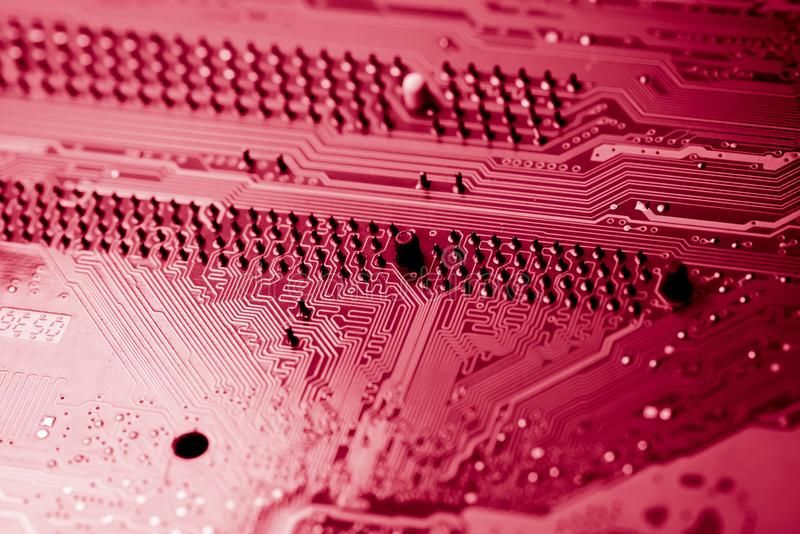
\includegraphics[height=\paperheight,width=\paperwidth]{../03_img/processor_red.jpg}
		};
	}
	\begin{frame}[plain]
		\begin{center}
			\begin{tcolorbox}[
				skin=enhanced,
	      			boxrule=0.6mm, boxsep=0mm,
				lowerbox=ignored,
				colback=orange!60!red, colframe=black,
				borderline={0.5pt}{3pt}{black}, borderline={1pt}{2pt}{red},
				width=\textwidth
			]
				\centering
				\Huge\textbf{\inserttitle}
			\end{tcolorbox}
			\vspace*{1.4cm}
			\begin{tcolorbox}[width=0.5\textwidth]
				\centering
				\textbf{\insertauthor} \\[2mm]
				\insertinstitute \\[2mm]
				\insertdate
			\end{tcolorbox}
			
			\begin{textblock}{1}(1,13.5)
				
\includegraphics[scale=0.04]{../03_img/logo_dhbw}
			\end{textblock}
		\end{center}
	\end{frame}}
}

% table of contents
\newcommand{\dwPrintToc}[1]{
	{\makeatletter
   		\setbeamertemplate{headline}[default]
   		\def\beamer@entrycode{\vspace*{-\headheight}}
	\makeatother

	\begin{frame}[allowframebreaks]
		\begin{tcolorbox}[
			skin=enhanced,
      			boxrule=0.6mm, boxsep=0mm,
			lowerbox=ignored,
			colback=orange!60!red, colframe=black,
			borderline={0.5pt}{3pt}{black}, borderline={1pt}{2pt}{red},
			width=\textwidth
		]
			\centering
			\huge\textbf{Agenda for this Unit}
		\end{tcolorbox}
		\vspace{2mm}
		
		{\renewcommand{\baselinestretch}{1.4}
		\tableofcontents}
	\end{frame}}
}

% hyperlinks
% ====================================================
% redefine cref (add a hyperlink)
\let\chyperref\cref % save original command under a new name
\renewcommand{\cref}[1]{\hyperlink{#1}{\textcolor{blue}{$\Rightarrow$ \chyperref{#1}}}}

\newcommand{\externalurl}[2]{\href{#1}{\textcolor{blue}{$\Rightarrow$ #2}}}


% ====================================================
% ====================================================
% OPTIONS
% ====================================================
% ====================================================

% number of levels in toc
\dwDeepToc{false}

\newcommand{\code}[2][fill=lightgray!50]{%
	\tikz[baseline]\node[%
        	inner ysep=0.5pt, 
        	inner xsep=2pt, 
        	anchor=text, 
        	rectangle, 
        	rounded corners=1mm,
        	#1] {\strut \texttt{#2}};%
}

% ====================================================
% ====================================================
% PRESENTATION DATA
% ====================================================
% ====================================================

\title[Introduction to Python for ML]{***** Introduction to Python for ML *****}
\author{Daniel Wehner, M.Sc.}
\institute[SAP\,SE]{SAP\,SE / DHBW Mannheim}
\date{Winter term 2020/2021}

% ====================================================
% ====================================================
% BEGIN OF DOCUMENT
% ====================================================
% ====================================================

\begin{document}

% Title frame
%______________________________________________________________________
\dwPrintTitle

% Agenda
%______________________________________________________________________
\dwPrintToc

% Section: Introduction
%______________________________________________________________________
\dwSection{Introduction}

% What is Python?
\begin{dwHeaderFrame}{What is Python?}
	\begin{itemize}
		\item Python was developed by Guido van Rossum in the early 1990s.
		\item It is an interpreted, high-level, general-purpose programming language which is the state-of-the-art for data science and machine learning.
		\item \textbf{White space has a meaning!} (important difference to other languages like Java or C++)
		\begin{itemize}
			\item Semantic code blocks (e.\,g. conditions, loops, ...) have to be indented.
			\item You may use tabs or spaces for indentation, but the interpreter \textbf{does not allow you to mix these two!}
		\end{itemize}
		\item Python supports many programming paradigms: We can write \textbf{procedural}, \textbf{functional} or \textbf{object-oriented} programs.
	\end{itemize}
\end{dwHeaderFrame}


\begin{frame}
	\begin{itemize}
		\item \textbf{Caveat:} Python has two \textbf{non-compatible} branches:
		\begin{itemize}
			\item \texttt{Python 2.7} $\Longleftarrow$ This one is deprecated and no longer maintained
			\item \texttt{Python 3.x} $\Longleftarrow$ Use this one!
		\end{itemize}
	\end{itemize}
\end{frame}


% Installation and Components
\begin{dwHeaderFrame}{Installation and Components}
	\dwHeader{Python}
	\begin{itemize}
		\item Python is pre-installed on Mac and Linux. You may check this by executing \texttt{python -V} in the command line.
		\item For Windows (and Mac), download the newst version from \externalurl{www.python.org/downloads/}{www.python.org/downloads/}.
		\item Don't forget to check the \texttt{`Add Python 3.x to PATH'} option!
	\end{itemize}
	\dwHeader{Jupyter}
	\begin{itemize}
		\item It is a browser-based Python environment (either on local or remote machine).
		\item The code is editable directly in the browser.
		\item Nice for (interactive) demonstrations, \textbf{but hard to debug}.
	\end{itemize}
\end{dwHeaderFrame}


\begin{frame}
	\dwHeader{Anaconda}
	\begin{itemize}
		\item A package manager for creating \textbf{isolated Python environments} (with different package versions)
		\item It is good programming practice to create separate environments for different projects in order to avoid version mismatches,
			package clashes etc.
		\item It can be downloaded from \externalurl{https://www.anaconda.com/download/}{https://www.anaconda.com/download/}
	\end{itemize}
	
	\dwInfoBox{I recommend to use the \textit{Anaconda Navigator} which combines all components, including a Python IDE called \textit{spyder}.}
\end{frame}


% Section: Variables and Data Types
%______________________________________________________________________
\dwSection{Variables and Data Types}

% Basic Data Types
\begin{dwHeaderFrame}{Basic Data Types}
	\begin{itemize}
		\item Unlike Java, Python is \textbf{typed dynamically}, i.\,e. the data type does not have to be specified when declaring variables.
		\item Nevertheless, Python works with these types internally (cf. \cref{tab:data_types}).
	\end{itemize}
	
	\dwTable{
	\begin{tabularx}{\textwidth}{ r | X | l }
		\textbf{Type} 	& \textbf{Description}  									& \textbf{Example}				\\ \hline
		\texttt{int} 	& Integer (no maximum for integers, only limited by memory size)		& 0, 1, 2, ...					\\ \hline
		\texttt{float} 	& Floating point number 									& 3.1415, 2.7182				\\ \hline
		\texttt{str}		& String (unicode characters) 								& `Hello world' 					\\ \hline
		\texttt{bool} 	& Boolean values 										& \texttt{True} or \texttt{False}
	\end{tabularx}
}{Basic data types in Python}{tab:data_types}{1.1}
\end{dwHeaderFrame}


\begin{frame}
	\dwHeader{Some examples}
	\lstinputlisting{00_intro_python/06_listings/data_types_string.txt}
\end{frame}


\begin{frame}{}
	\dwHeader{Conversion between Types}
	\begin{itemize}
		\item Although you don't have to bother with types in Python, you may want to convert a variable to another type.
		\item E.\,g. when concatenating a number to a string
	\end{itemize}
	
	\lstinputlisting{00_intro_python/06_listings/type_conversion.txt}
\end{frame}


\begin{frame}
	\dwHeader{Immutable data types}
	\lstinputlisting{00_intro_python/06_listings/immutable_data_types.txt}
\end{frame}


% Sequence Data Types
\begin{dwHeaderFrame}{Sequence Data Types}
	\begin{itemize}
		\item Sometimes it is necessary to store multiple elements in one place.
			Think e.\,g. of a list of data points which we want to analyze using machine learning methods.
		\item Python offers the types \code{range}, \code{list} and \code{tuple} for that. 
	\end{itemize}
	
	\dwHeader{Ranges}
	\begin{itemize}
		\item The \code{range} type represents an immutable sequence of numbers and is commonly used for looping a specific number of times in for-loops.
		\item \textbf{Interface:} class \texttt{range}(\textit{start}, \textit{stop}[, \textit{step}])
		\begin{itemize}
			\item \textit{start}: Fist point in the sequence of numbers (default = 0).
			\item \textit{stop}: Last point in the sequence of numbers (excluding).
			\item \textit{step}: Step size
		\end{itemize}
	\end{itemize}
\end{dwHeaderFrame}
	
	
\begin{frame}
	\dwHeader{Lists}
	\begin{itemize}
		\item Lists are \textbf{mutable} sequences of elements (i.\,e. elements can be inserted, modified, deleted).
		\item Lists can be constructed in several ways:
		\begin{itemize}
			\item Using a pair of square brackets (empty list): \code{[]}
			\item Using square brackets, separating items with commas: \code{[a]}, \code{[a, b, c]}
			\item Using the type constructor: \code{list()} or \code{list(iterable)}
			\item Using a \textbf{list comprehension}: \code{[x for x in iterable]}
		\end{itemize}
		\item Example: \code{list(range(1, 10)) = [1, 2, 3, 4, 5, 6, 7, 8, 9]}
	\end{itemize}
	
	\dwInfoBox{Lists are commonly used to store \textit{homogeneous} types of elements, e.\,g. a list of customers.}
\end{frame}


\begin{frame}
	\begin{itemize}
		\item List comprehensions originate from \textbf{functional programming} and provide a concise way to create lists.
		\item Common applications are to make new lists where each element is the result of some operations applied to each member of
			another sequence or iterable, or to create a subsequence of those elements that satisfy a certain condition.
		\item Example: Compute square numbers:
	\end{itemize}
	
	\lstinputlisting{00_intro_python/06_listings/list_comprehensions.txt}
	\dwInfoBox{Task: Create a list of prime numbers up to $n$ by using list comprehensions only!}
\end{frame}


\begin{frame}
	\dwHeader{Excursion: Sets}
	\begin{itemize}
		\item Python also includes a data type for sets.
		\item Following the mathematical notion of a set, it is an \textbf{unordered} collection with \textbf{no duplicate} elements.
		\item A set can be created using \code{set()} (not \code{\{\}}!)
		\item \code{set([4, 1, 2, 2, 6])} gives \code{\{ 1, 2, 4, 6 \}}
		\item \code{set([4, 1, 2, 2, 6]) == set([4, 4, 4, 1, 2, 6, 2])} evaluates to \code{True}!
	\end{itemize}
\end{frame}


\begin{frame}
	\dwHeader{Tuples}
	\begin{itemize}
		\item Tuples are \textbf{immutable} sequences, typically used to store collections of \textbf{heterogeneous} data (it is not enforced, though).
		\item Think e.\,g. of a customer record which includes the name, address and contact.
		\item Tuples can be constructed in several ways:
		\begin{itemize}
			\item Using a pair of parentheses (empty tuple): \code{()}
			\item Using a trailing comma for a singleton tuple: \code{a,} or \code{(a,)}
			\item Separating items with commas: \code{a, b, c} or \code{(a, b, c)}
			\item Using the \code{tuple()} built-in: \code{tuple()} or \code{tuple(iterable)}
		\end{itemize}
	\end{itemize}
\end{frame}


% Mapping Types
\begin{dwHeaderFrame}{Mapping Types}
	\begin{itemize}
		\item A mapping object maps hashable values to arbitrary objects.
		\item Mappings are \textbf{mutable} objects.
		\item There is currently only one standard mapping type, the \textbf{dictionary} -- \code{dict}.
		\item A dictionary consists of key-value pairs. Consider it to be a telephone book where the keys are the names and the values are the numbers.
		\item A dictionary’s keys are almost arbitrary values. Values that are not hashable, that is, values containing lists,
			dictionaries or other mutable types (that are compared by value rather than by object identity) may \textbf{not} be used as keys.
		\item Dictionaries can be created in two ways:
		\begin{itemize}
			\item A comma-separated list of key-value pairs: \code{\{ key1: value1, key2: value2, ... \}}
			\item By using the \code{dict()} constructor.
		\end{itemize}
	\end{itemize}
\end{dwHeaderFrame}


\begin{frame}
	\lstinputlisting{00_intro_python/06_listings/dicts.txt}
\end{frame}


% Section: Logical Operators
%______________________________________________________________________
\dwSection{Logical Operators}

% Basic Data Types
\begin{dwHeaderFrame}{Logical Values}
	\begin{itemize}
		\item Logical constants in Python: \code{True} and \code{False}.
		\item The value of a logical expression is false, if it returns one of the following:
		\begin{itemize}
			\item The \code{False} constant.
			\item The \code{None} object.
			\item An empty sequence or collection: \code{[]}, \code{()}, \code{`'} ...
			\item The number 0.
		\end{itemize}
		\item Everything else evaluates to \code{True}.
	\end{itemize}
\end{dwHeaderFrame}


\begin{frame}
	\dwTable{
	\begin{tabularx}{\textwidth}{ X | X | X}
		\textbf{Operator} & \textbf{Description} & \textbf{Example} 		\\ \hline
		< 		&	less than 				& 	\code{5 < 7}		\\ \hline
		<= 		& 	less than or equal to 		& 	\code{5 <= 7} 		\\ \hline
		== 		& 	equal to 				& 	\code{3 == (2 + 1)} 	\\ \hline
		!= 		&	not equal to 			& 	\code{4 != 42} 		\\ \hline
		>=		& 	greater than or equal to 	& 	\code{6 >= 6}		\\ \hline
		> 		& 	greater than 			& 	\code{9 > 8} 		\\ \hline\hline
		or		& 	logical or 				& 	\code{a or b} 		\\ \hline
		and 		& 	logical and 			& 	\code{a and b} 		\\ \hline
		not 		& 	logical negation 			& 	\code{not a} 		\\ \hline
		(not) in 	& 	containment 			& 	\code{2 in [3, 6, 2]} 	\\ \hline
		(not) is	& 	identity operator 		& 	\code{a is b}
	\end{tabularx}
}{Logical operators in Python}{tab:data_types}{1.4}
\end{frame}


% Section: Control Flow
%______________________________________________________________________
\dwSection{Control Flow}

% Conditionals
\begin{dwHeaderFrame}{Conditionals}
	\begin{itemize}
		\item Conditionals are used to branch program execution based on conditions.
		\item \textbf{Indentation is important to define the scope!} If you forget the indentation,
			Python will give you a hint stating that it expects an indented block.
		\item General form of a conditional:
	\end{itemize}
	
	\lstinputlisting{00_intro_python/06_listings/conditionals.txt}
\end{dwHeaderFrame}


% Loops
\begin{dwHeaderFrame}{Loops}
	\begin{itemize}
		\item Loops are used to repetitively execute code (and save a large amount of effort and time).
		\item Python basically distinguishes between two types of loops: The \code{while}-loop and the \code{for}-loop.
			One type of loop can be expressed in terms of the other (\textbf{syntactical sugar}).
	\end{itemize}
	
	\dwHeader{While-loops}
	\begin{itemize}
		\item With the \code{while}-loop we can execute a set of statements as long as a condition is true.
		\item It requires the relevant variables to be initialized (\code{i} in the example below).
		\item Typically used when the number of iterations is not known in advance.
	\end{itemize}
	
	\lstinputlisting{00_intro_python/06_listings/while_loop.txt}
\end{dwHeaderFrame}


\begin{frame}
	\dwHeader{For-loops}
	\begin{itemize}
		\item \code{for}-loops are typically used when the number of iterations is known in advance / when iterating over collections.
		\item The implementation differs from what you know from Java or C.
	\end{itemize}
	
	\lstinputlisting{00_intro_python/06_listings/for_loop.txt}
\end{frame}


% Section: Python OO
%______________________________________________________________________
\dwSection{Python OO}

% Classes
\begin{dwHeaderFrame}{What are Classes?}
	\begin{itemize}
		\item Classes provide a means of bundling data and functionality together.
		\item A class consists of \textbf{attributes} and \textbf{methods}.
		\item \textbf{Definition of a simple class:}
	\end{itemize}
	
	\lstinputlisting{00_intro_python/06_listings/class_definition.txt}
\end{dwHeaderFrame}


\begin{frame}
	\begin{itemize}
		\item Classes are instantiated like this: \code{x = MyClass()}.
		\item Attributes and methods can be accessed using the \textbf{dot-operator}.
		\begin{itemize}
			\item Read attribute: \code{print(x.i)}, write attribute: \code{x.i = 123}
			\item Call method: \code{x.f()}
		\end{itemize}
		\item By default, all class members (attributes and methods) are \textbf{public}. \textbf{Private members do not exist in Python}.
			\textit{But: Cf. \textit{name mangling}}
		\item Each class implicitly contains some built-in methods (not exhaustive):
		\begin{table}
			\centering
			\renewcommand{\arraystretch}{2.0}
			\begin{tabular}{ l l l l }
				\textbullet 		& 	\textbf{Constructor:} 		& 	\code{\_\_init\_\_(self):}		&	Passes initial state to object 	\\
				\textbullet 		& 	\textbf{Hash:} 			& 	\code{\_\_hash\_\_(self):}		& 	Defines the hash of the object 	\\
				\textbullet 		& 	\textbf{Equality:} 		& 	\code{\_\_eq\_\_(self, other):} 	&	Comparison with other objects	\\
			\end{tabular}
		\end{table}
	\end{itemize}
\end{frame}


% Class Variables vs. Instance Variables
\begin{dwHeaderFrame}{Class Variables vs. Instance Variables}
	\begin{itemize}
		\item Class variables are shared by all objects / instances of that class.
		\item Instance variables are for data unique to each object / instance. Such variables are declared using \code{self.var\_name}.
		\item Cf. next slide for an example.
	\end{itemize}
\end{dwHeaderFrame}


\begin{frame}
	\lstinputlisting{00_intro_python/06_listings/instance_class_var.txt}
\end{frame}


% Inheritance
\begin{dwHeaderFrame}{Inheritance}
	\begin{itemize}
		\item The syntax for class inheritance is \code{class sub\_class\_name(base\_class\_name):}
		\item Python allows for \textbf{polymorphism} (all methods are \textbf{virtual}).
		\item Python also supports some form of multiple inheritance.
	\end{itemize}
\end{dwHeaderFrame}


% Section: Machine Learning Libraries
%______________________________________________________________________
\dwSection{Machine Learning Libraries}

% NumPy
\begin{dwHeaderFrame}{NumPy}
	\begin{itemize}
		\item NumPy (Numerical Python) is the fundamental package for scientific computing with Python.
			It is mostly implemented in C and therefore \textbf{very fast}.
		\item It is a library which defines \textbf{multidimensional array objects} (\code{ndarray}) along with functions / routines
			that can operate on those arrays.
		\item The package includes routines for \textbf{linear algebra}, random number generation and many others.
		\item Install the package using \code{pip install numpy}.
	\end{itemize}
\end{dwHeaderFrame}


\begin{frame}
	\dwHeader{ndarray}
	\begin{itemize}
		\item The most important object in NumPy.
		\item Creation of ndarrays (assume: \code{import numpy as np}):
		\begin{itemize}
			\item 0-dimensional: np.array(42)
			\item 1-dimensional: np.array([1, 2, 3])
			\item 2-dimensional: np.array([[1, 2], [3, 4], [5, 6]])
			\item 3-dimensional: np.array([[[1, 2], [3, 4]], [[5, 6], [7, 8]]])
			\item ...
		\end{itemize}
		\item \textcolor{blue}{\textit{What do we call the above objects from a mathematical point of view?}}
		\item If you are interested in the dimensionality of an array you can use \code{ndarray.shape}, e.\,g.: \\
			\code{np.array([[1, 2, 3], [3, 8, 6]]).shape} gives \code{(2, 3)} -- 2 rows, 3 columns.
	\end{itemize}
\end{frame}


\begin{frame}
	\dwHeader{Creation of arrays}
	\begin{itemize}
		\item \textbf{Creation of arrays from scratch:}
		\begin{itemize}
			\item \code{np.empty(shape)}: Creates an empty array (not initialized). It is filled with random numbers.
			\item \code{np.zeros(shape)}: Creates an array of zeros.
			\item \code{np.ones(shape)}: Creates an array of ones.
		\end{itemize}
	\end{itemize}
	\dwAlertBox{The creation of an empty array can lead to strange errors later in your code. I recommend to use the second or third method instead.}
	
	\begin{itemize}
		\item \textbf{Creation of arrays from existing data:}
		\begin{itemize}
			\item \code{np.array(data)}: Creates a copy of \code{data} and converts the copy to an array.
			\item \code{np.asarray(data)}: Uses the original data, changes to the array are reflected in the original data.
		\end{itemize}
	\end{itemize}
\end{frame}


\begin{frame}
	\dwHeader{Indexing}
	\begin{itemize}
		\item \textbf{Standard indexing:}
		\begin{itemize}
			\item Indexing in NumPy is rather simple (in fact it is very similar to standard lists).
			\item This gives you the \textbf{sixth} element from the array: \code{arr[5]} (\textbf{zero-based index!}).
			\item Further dimensions are separated with a comma: \code{arr[5,3]} (fifth row, third column).
			\item A complete row (here: the first one) can be retrieved by: \code{arr[0,:]} or \code{arr[0,...]}
		\end{itemize}
		\item \textbf{Integer indexing:}
	\end{itemize}
	
	\lstinputlisting{00_intro_python/06_listings/integer_indexing.txt}
\end{frame}


\begin{frame}
	\dwHeader{Mathematical operations on arrays (by far not exhaustive!)}
	\vspace*{2mm}
	In the following consider two vectors \code{a = np.array([1, 3, 2])}, \code{b = np.array([4, 1, 0])} and the matrix \code{A = np.array([[1, 3], [3, 1]])}.
	\vspace*{2mm}
	\begin{table}
		\centering
		\renewcommand{\arraystretch}{2.0}
		\begin{tabular}{ l l l l }
			\textbullet & \textbf{Addition:} 		& \code{a + b = np.array([5, 4, 2])} 		& 									\\
			\textbullet & \textbf{Subtraction:} 	& \code{a - b = np.array([-3, 2, 2])} 		& 									\\
			\textbullet & \textbf{Multiplication:} 	& \code{a * b = np.array([4, 3, 0])} 		& \textit{(Hadamard/element-wise product)}	\\
			\textbullet & \textbf{Division:} 		& \code{a / b = np.array([0.25, 3, inf])} 	& 									\\
			\textbullet & \textbf{Inner product:} 	& \code{a @ b = 7} or \code{a.dot(b) = 7}	& \textit{(scalar product)} 					\\
			\textbullet & \textbf{Transpose:} 	& \code{A.T} 						& \textit{(swaps rows and columns)} 			\\
			\textbullet & \textbf{Matrix inverse:} 	& \code{np.linalg.inv(A)} 				& 									\\
		\end{tabular}
	\end{table}
\end{frame}


\begin{frame}
	\dwHeader{Broadcasting}
	\begin{itemize}
		\item The term broadcasting describes how NumPy treats arrays with different shapes during arithmetic operations.
		\item Subject to certain constraints, the smaller array is `broadcast' across the larger array so that they have compatible shapes.
		\item Broadcasting provides a means of \textbf{vectorizing} array operations so that looping occurs in C instead of Python.
		\item NumPy operations are usually done on pairs of arrays on an element-by-element basis:
	\end{itemize}
	\lstinputlisting{00_intro_python/06_listings/broadcasting_intro.txt}
	\begin{itemize}
		\item NumPy’s broadcasting rule \textbf{relaxes this constraint when the arrays’ shapes meet certain constraints}.
		The simplest broadcasting example occurs when an array and a scalar value are combined in an operation:
	\end{itemize}
	\lstinputlisting{00_intro_python/06_listings/broadcasting_example_1.txt}
\end{frame}


\begin{frame}
	\begin{itemize}
		\item NumPy compares the shapes of the arrays element-wise starting with trailing dimensions.
		\item Two dimensions are compatible when
		\begin{itemize}
			\item they are equal,
			\item or one of them is 1.
		\end{itemize}
		\item If these conditions are not met, a \code{ValueError: operands could not be broadcast together} exception is thrown,
			indicating that the arrays have incompatible shapes.
		\item The size of the resulting array is the maximum size along each dimension of the input arrays.
		\item Check out the \externalurl{https://docs.scipy.org/doc/numpy/user/basics.broadcasting.html}{NumPy documentation}!
	\end{itemize}
\end{frame}


% ScikitLearn
\begin{dwHeaderFrame}{ScikitLearn}
	\begin{itemize}
		\item scikit-learn is a Python module for machine learning built on top of SciPy.
		\item The project was started in 2007 by David Cournapeau as a Google Summer of Code project, and since then many volunteers have contributed.
		\item The library implements all common machine learning algorithms (classification, regression, clustering, dimensionality reduction)
			with a standardized API.
		\item Furthermore, functionality for model selection and data pre-processing is included.
		\item Install the library with \code{pip install scikit-learn}
		\item Standard methods all algorithms implement:
		\begin{itemize}
			\item \code{model.fit(X\_train, y\_train)}: Fits the model to the training data. This is called \textbf{training}.
			\item \code{model.predict(X\_test)}: Uses the trained model to get predictions for \textbf{unseen data}.
		\end{itemize}
	\end{itemize}
\end{dwHeaderFrame}


\begin{frame}
	\dwHeader{General procedure}
	\lstinputlisting{00_intro_python/06_listings/scikit_learn_procedure.txt}
\end{frame}


\begin{frame}
	\begin{itemize}
		\item \code{X\_train} must be a two-dimensional array of features: \code{np.array([[...], [...], ...])}.
		\item \code{y\_train} is a one-dimensional array of corresponding class labels, e.\,g.: \code{np.array([0, 1, 1, 0, ...])}
	\end{itemize}
	
	\dwInfoBox{Task: Install scikit-learn and try it for yourself!}
\end{frame}


% Matplotlib
\begin{dwHeaderFrame}{Matplotlib (PyPlot)}
	\begin{itemize}
		\item \code{matplotlib.pyplot} is a collection of command style functions that make matplotlib work like MATLAB.
		\item Each pyplot function makes some change to a figure: e.g., creates a figure, creates a plotting area in a figure,
			plots some lines in a plotting area, decorates the plot with labels, etc.
		\item Generating visualizations with pyplot is very quick (plot on next slide):
	\end{itemize}
	\lstinputlisting{00_intro_python/06_listings/pyplot_example_1.txt}
\end{dwHeaderFrame}


\begin{frame}
	\dwFigure{
		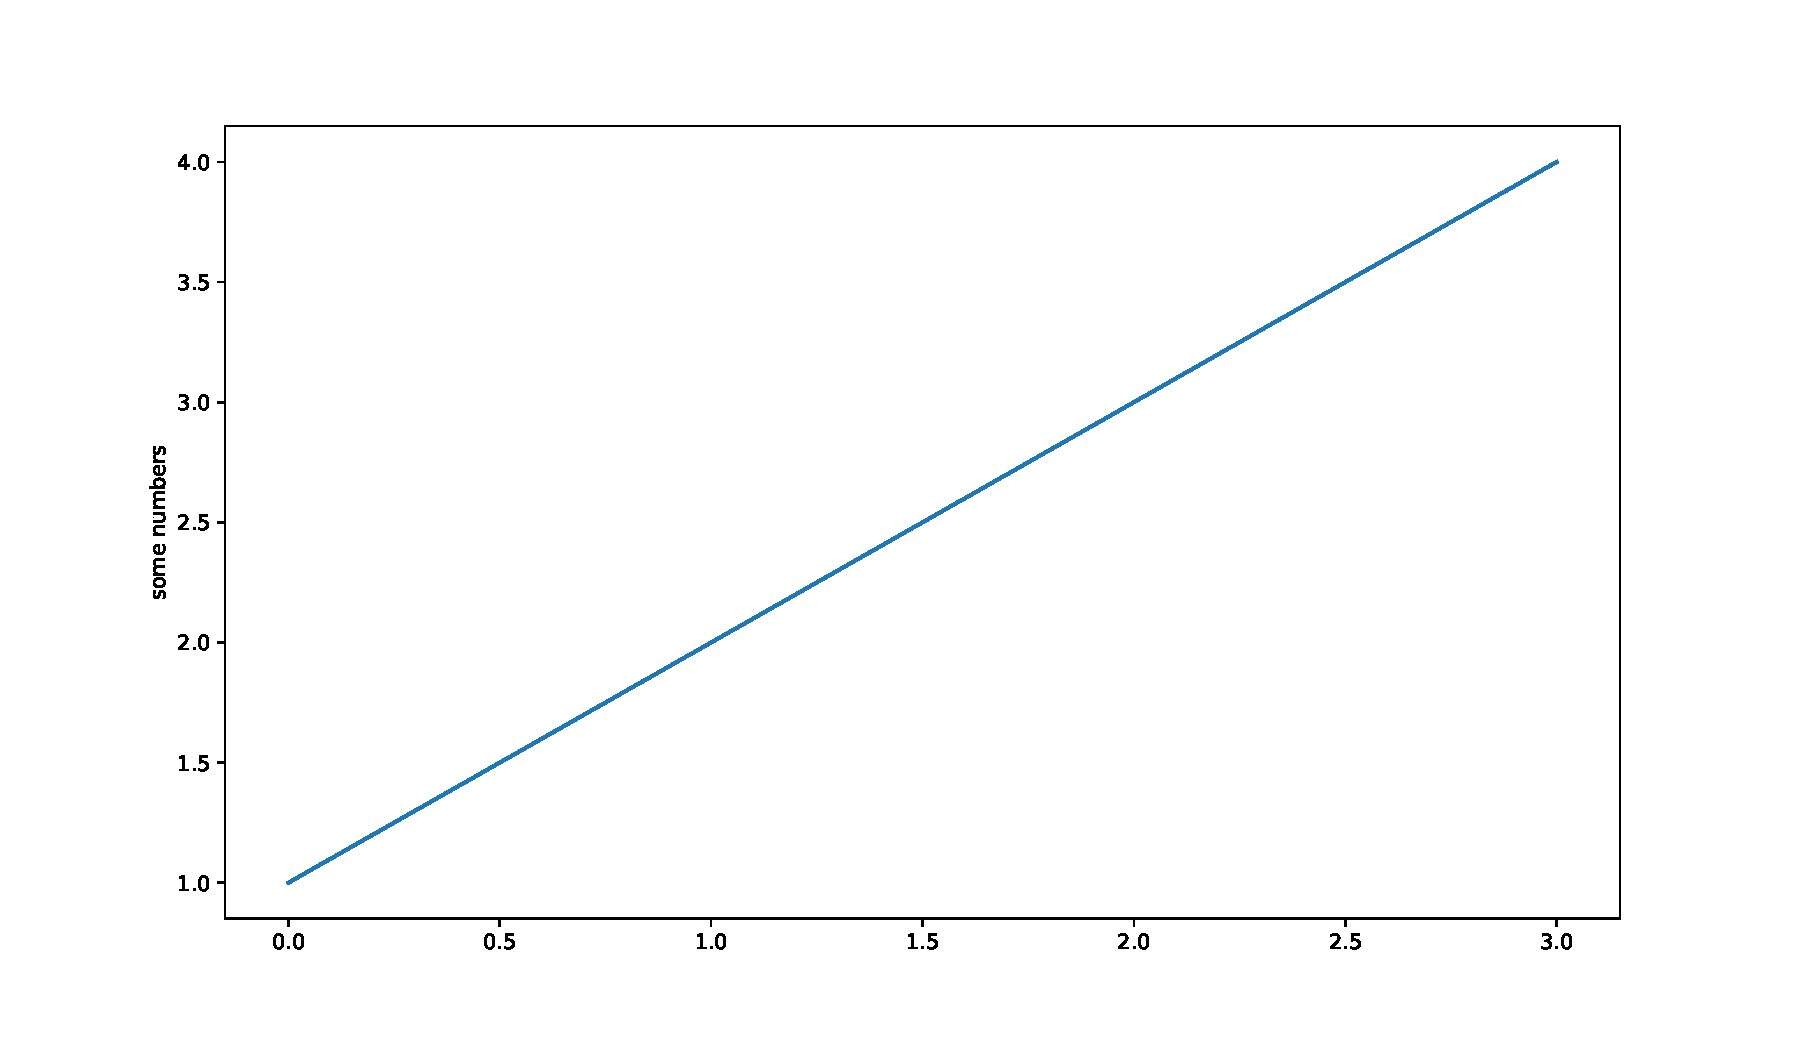
\includegraphics[scale=0.325]{00_intro_python/02_img/pyplot_example_1}	
	}{Simple pyplot example}{fig:pyplot-example-1}
\end{frame}


\begin{frame}
	\begin{itemize}
		\item Plotting in different colors and shapes is quite easy. Some colors and shapes are predefined and can be accessed using string-constants,
			cf. \code{r--} (red dashed), \code{bs} (blue squares) and \code{g\^} (green triangles) below.
		\item Also, Numpy and pyplot go hand in hand:
	\end{itemize}
	\lstinputlisting{00_intro_python/06_listings/pyplot_example_2.txt}
	
	\dwInfoBox{matplotlib.pyplot can handle NumPy arrays! This is very useful, since NumPy arrays are omnipresent in machine learning applications.}
\end{frame}


\begin{frame}
	\dwFigure{
		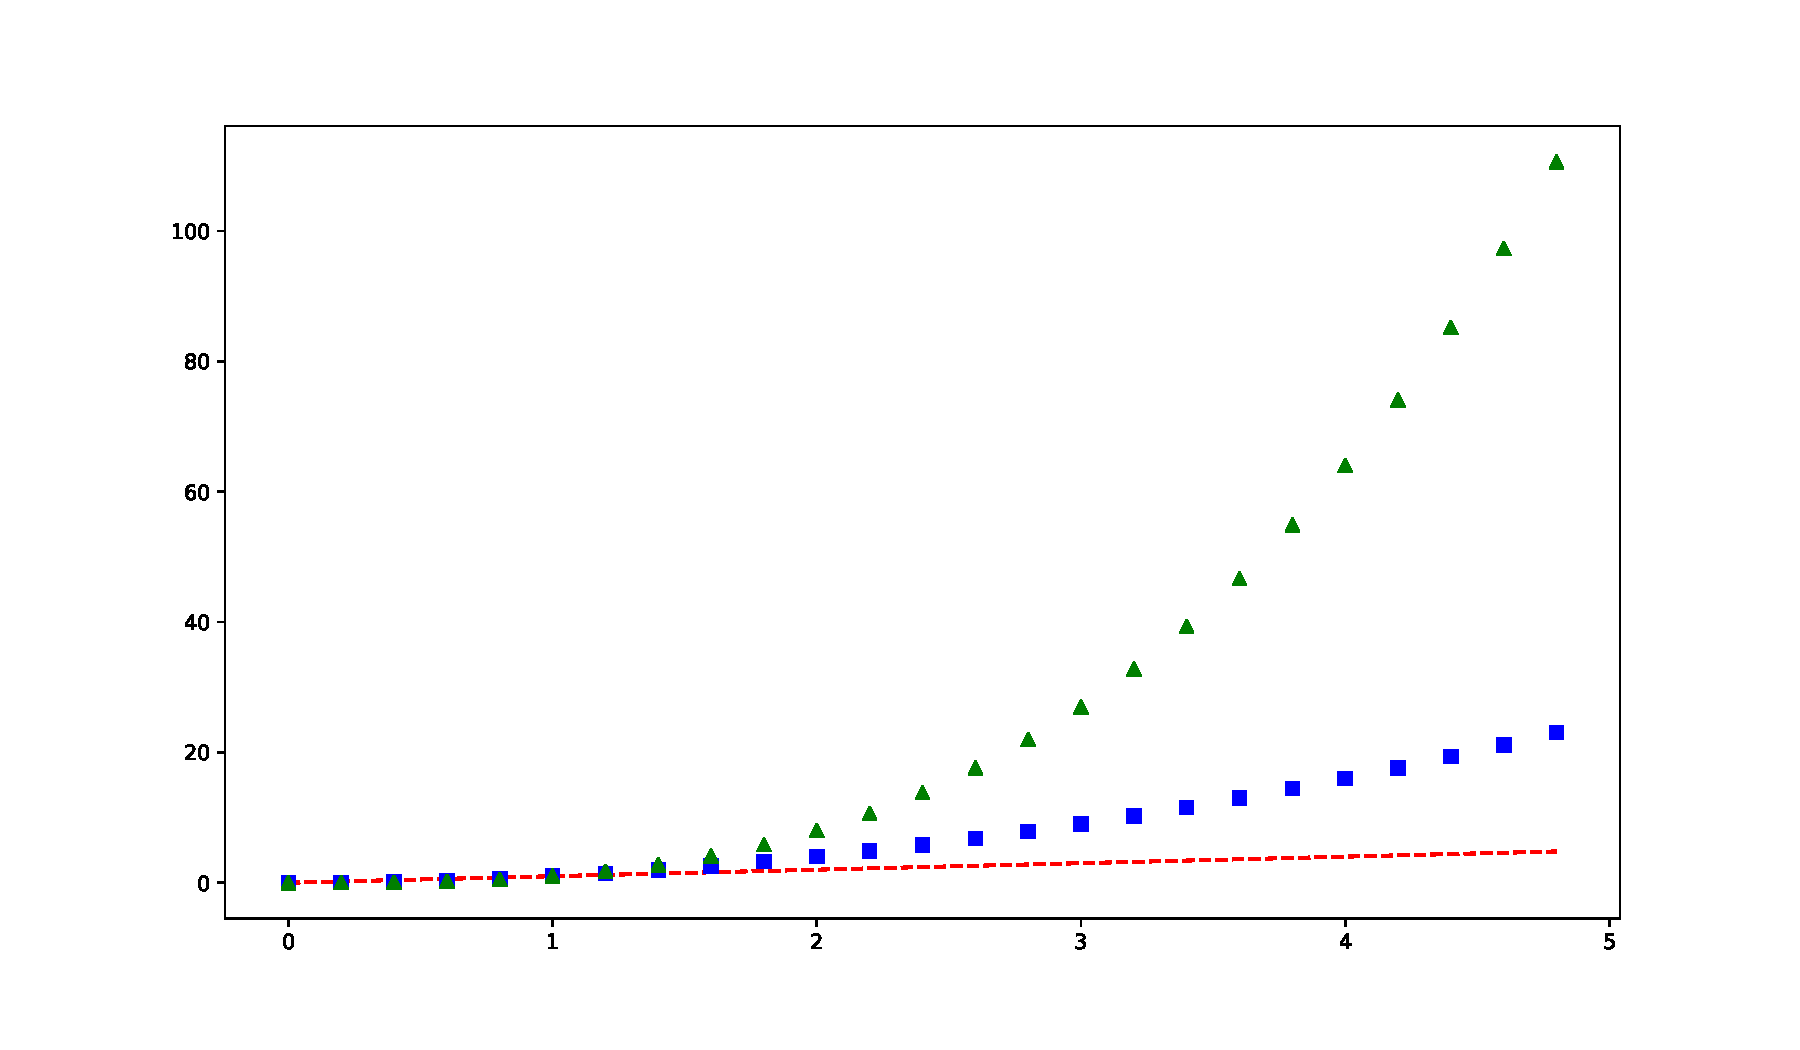
\includegraphics[scale=0.325]{00_intro_python/02_img/pyplot_example_2}	
	}{A more sophisticated pyplot example}{fig:pyplot-example-2}
\end{frame}


\begin{frame}
	\dwHeader{Plotting contours}
	\begin{itemize}
		\item Contour plots can be useful for plotting decision boundaries of classifiers.
		\item For that you have to create a mesh-grid and classify all points in the grid with your classifier. Matplotlib then assigns a color
			to that point based on the classification result.
		\item Let use make a step-by-step example: 
	\end{itemize}
\end{frame}


\begin{frame}
	\lstinputlisting{00_intro_python/06_listings/pyplot_contours_1.txt}
\end{frame}


\begin{frame}
	\lstinputlisting{00_intro_python/06_listings/pyplot_contours_2.txt}
\end{frame}


\begin{frame}
	\dwFigure{
		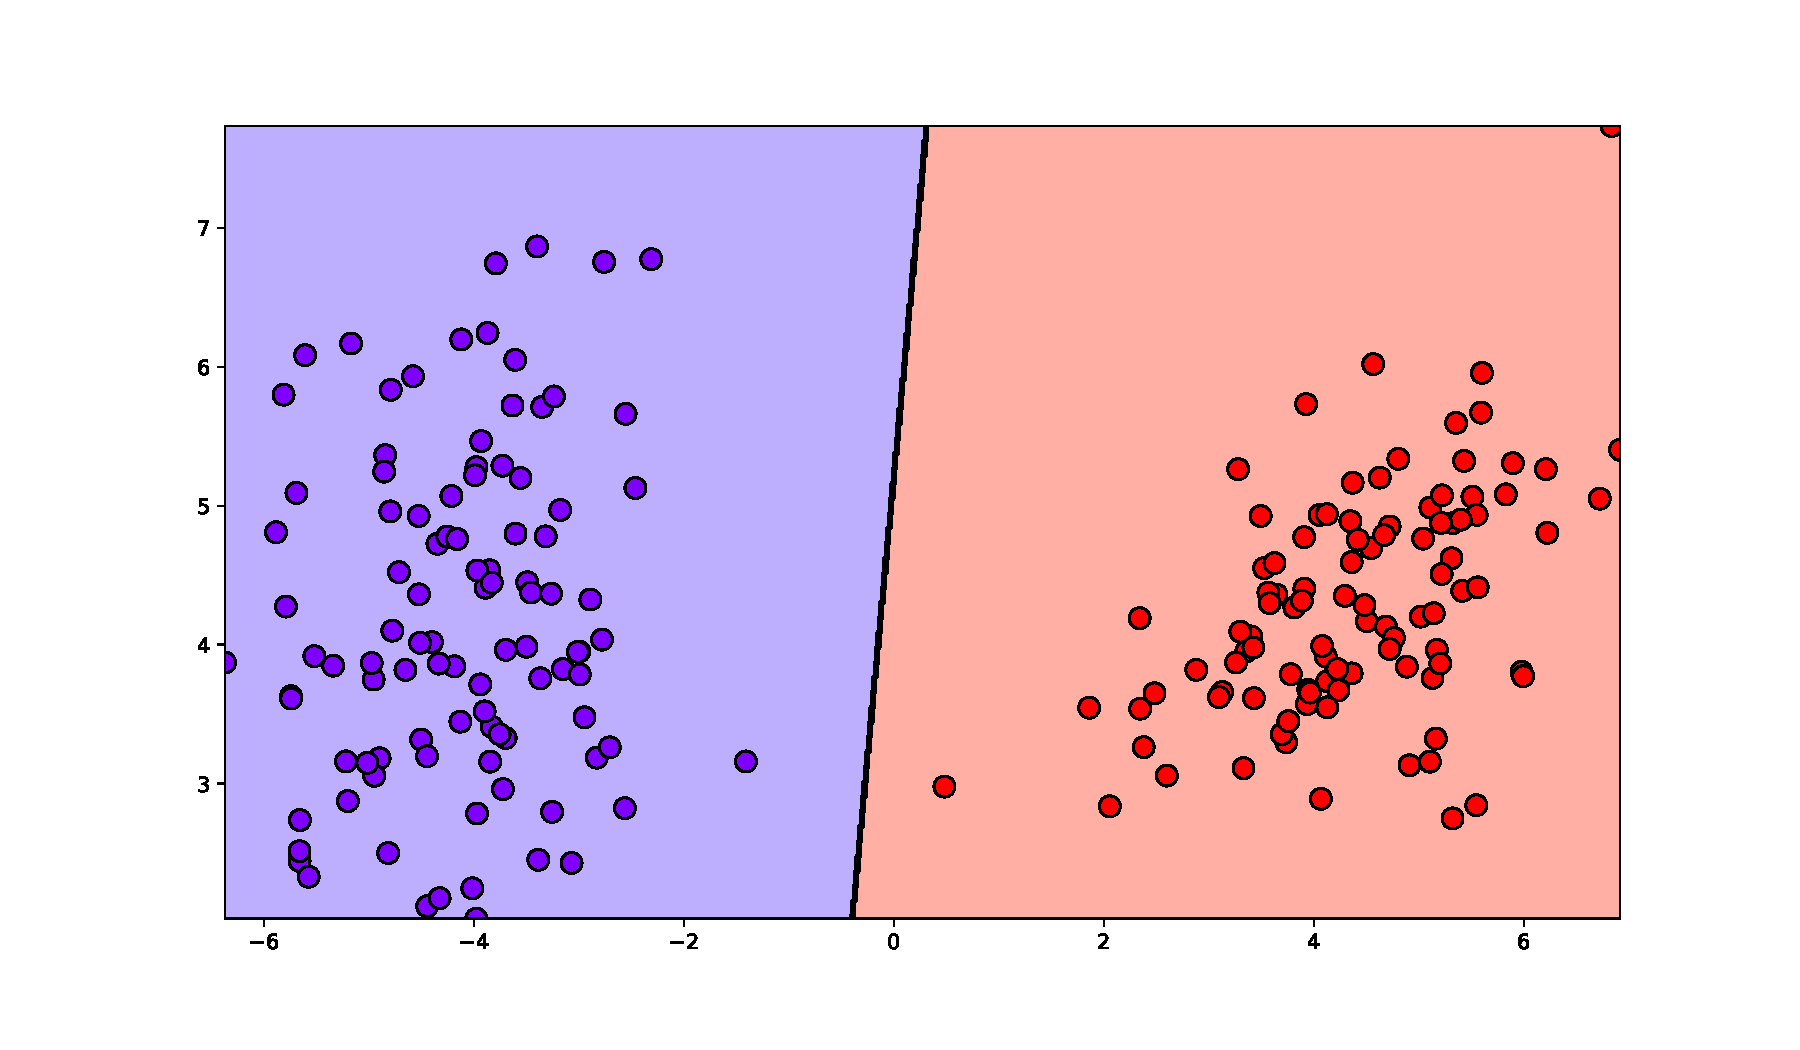
\includegraphics[scale=0.325]{00_intro_python/02_img/contour}	
	}{A contour plot in matplotlib}{fig:contour}
\end{frame}


% PyTorch
\begin{dwHeaderFrame}{PyTorch}
	\begin{itemize}
		\item
	\end{itemize}
\end{dwHeaderFrame}


% Thank you
%______________________________________________________________________
\makethanks

\end{document}
